% !TeX TXS-program:compile = txs:///pdflatex/[--shell-escape]
% !TeX root = gnn-pres
% !TeX encoding = UTF-8
% !TeX spellcheck = en_US
% https://orcid.org/0000-0003-4586-8500


%\documentclass[14pt]{beamer}
\documentclass[aspectratio=169]{beamer} % Other possible values are: 1610, 149, 54, 43 and 32. By default, it is to 128mm by 96mm(4:3)

\documentclass{article}
\usepackage{blindtext}

%%% FONTS %%%
\usepackage[T1]{fontenc}
\usepackage[utf8]{inputenc}
\usepackage[english]{babel}
%\usepackage{tgpagella} % set the document font to TeX Gyre Pagella
%\usepackage{tgbonum} % set the document font to TeX Gyre Bonum
%\usepackage{fontawesome5} % The Creative Commons icons

%%% DRAFT watermark %%%
\usepackage{draftwatermark}
\SetWatermarkText{DRAFT}
\SetWatermarkScale{5.1}
\SetWatermarkLightness{0.8}

\usepackage{xcolor} % \textcolor{red}{text} will be red for notes
\definecolor{lightgray}{gray}{0.6}
\definecolor{medgray}{gray}{0.4}

\usepackage{hyperref}
\hypersetup{
	colorlinks=true,
	urlcolor= blue,
	citecolor=blue,
	linkcolor= blue,
	%bookmarks=true,
	%bookmarksopen=false,
}

% Code to add paragraph numbers and titles
\newif\ifptitle
\newif\ifpnumber
\newcounter{para}
\newcommand\ptitle[1]{\par\refstepcounter{para}
	{\ifpnumber{\noindent\textcolor{lightgray}{\textbf{\thepara}}\indent}\fi}
	{\ifptitle{\textbf{[{#1}]}}\fi}}
\ptitletrue  % comment this line to hide paragraph titles
\pnumbertrue  % comment this line to hide paragraph numbers

% for inserting images in line
\usepackage{graphicx}
\graphicspath{ {code/} }

%\usepackage[verbose]{wrapfig} % wrap text around image

\definecolor{myblue}{HTML}{4285F4} % color table cells

\usepackage[tablegrid]{vhistory} % version history package


% Allows to rewrite the same title in the supplement
\newcommand{\mytitle}{Analysis and Optimization of Security Infrastructure with Deep Learning Methods}
\usepackage{authblk}
\usepackage{comment} % allows block comments

\usepackage{ragged2e} % use flush and justify for text blocks
\usepackage{csquotes} % use \displayquote{} in the doc

%%% GRAPHICS  AND CODE BLOCKS %%%
\usepackage[listings, minted]{tcolorbox}
\usepackage{xcolor,colortbl}
\definecolor{myblue}{RGB}{0,163,243}
\definecolor{mygrey}{RGB}{128,128,128}
\definecolor{whitesmoke}{RGB}{245,245,245}
\newtcolorbox[auto counter, number within=section]{mybox}[2][]{
	colbacktitle=mygrey,
	colback=whitesmoke,
	title={#2},
	fonttitle=\ttfamily\small,
	fontupper=\sffamily\small,
	halign=flush left,
	rounded corners
}

% Headers and footers
\usepackage{fancyhdr}
\pagestyle{fancy}
\fancyhf{}
\lhead{\mytitle}
\lfoot{\tiny{November 20, 2021}}
\rfoot{\tiny{version: \vhCurrentVersion}}

\usepackage{glossaries}
	\makeglossaries

\newacronym{Edge}{Edge}{define edge}
\newacronym{GitOps}{GitOps}{Implementing  version control, collaboration, compliance, and CI/CD tooling for infrastructure automation}
\newacronym{Node}{Node}{define a node}
\newacronym{Scalar}{Scalar}{define a scalar here}
\newacronym{Vector}{Vector}{define a vector here}

\newcommand*{\myglossaryindent}{0.65cm}
\newcommand*{\myglsdescwidth}{10cm}



% Table of Contents at Section start
\AtBeginSection[]
{
    \begin{frame}
        \frametitle{\bfseries\Huge\textcolor{black}{.}}
        \tableofcontents[currentsection]
    \end{frame}
}

\begin{document}

%%% Title Slide %%%
\usebackgroundtemplate{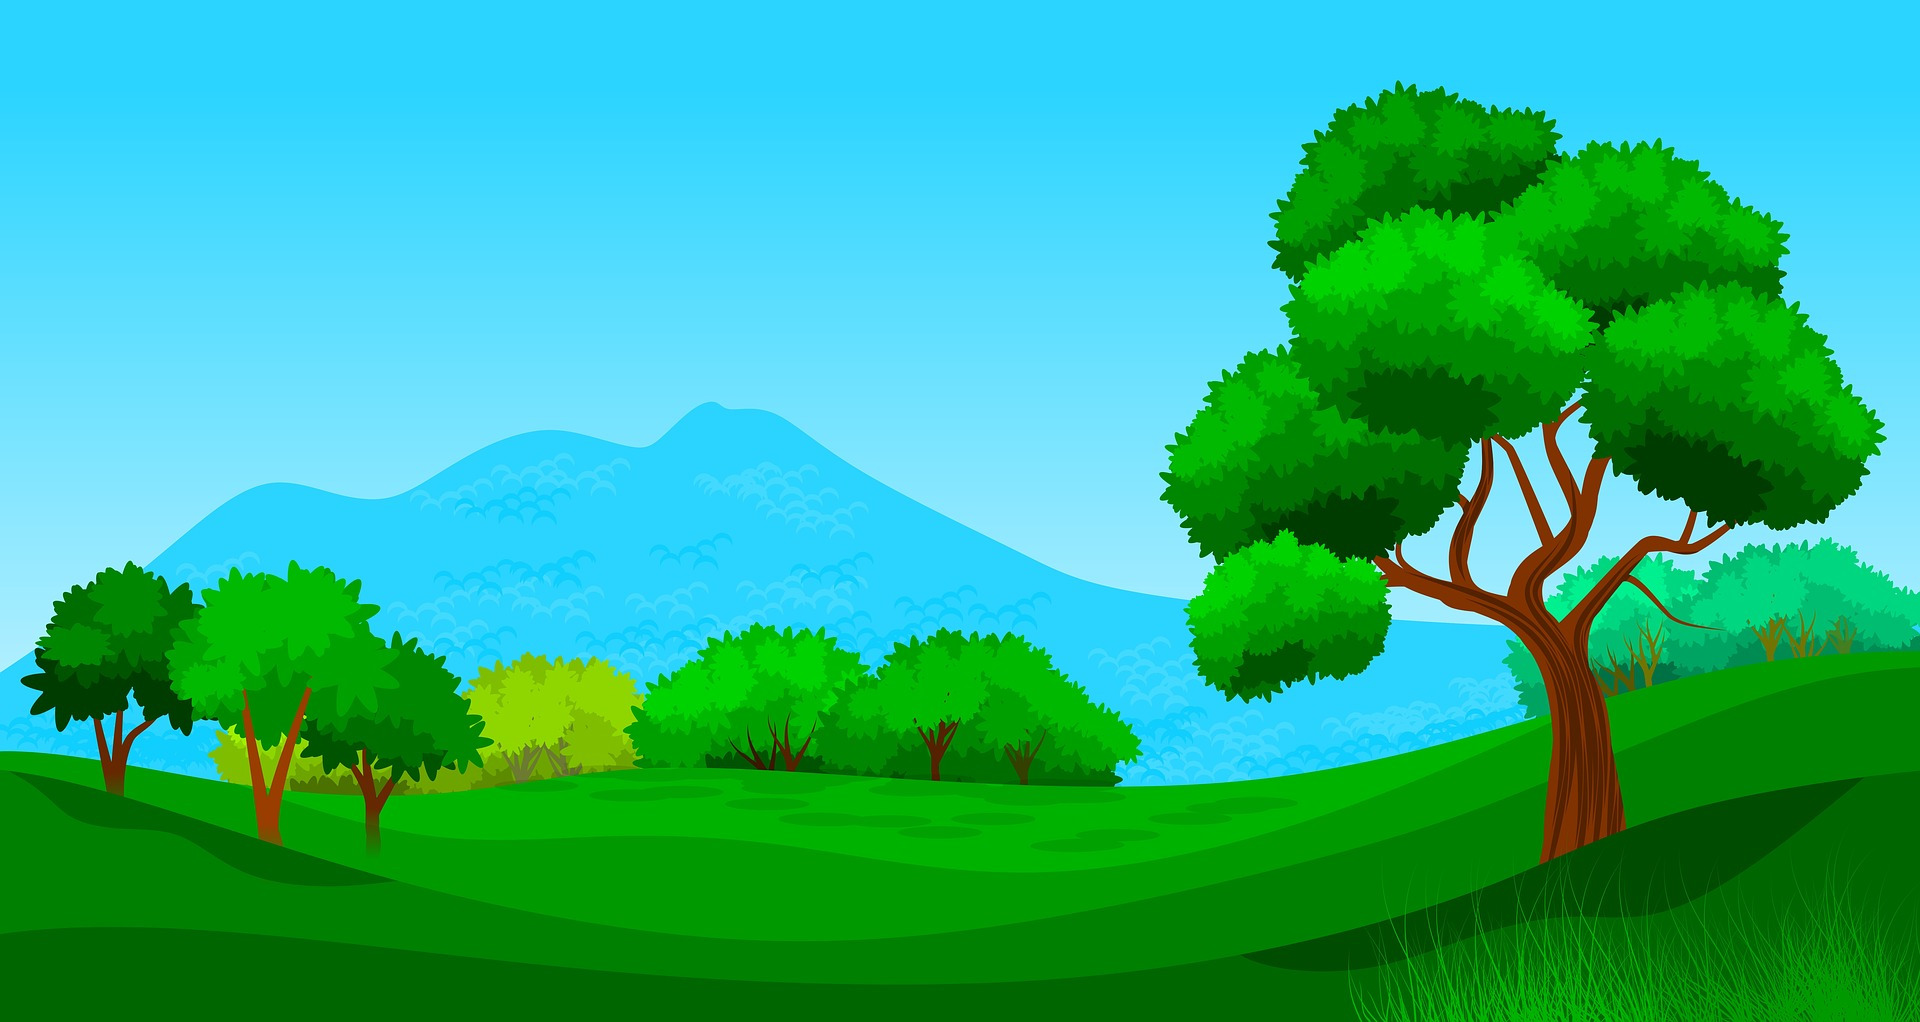
\includegraphics[width=\paperwidth]{../images/landscape.jpg}}
\begin{frame}
    \setlength{\TPHorizModule}{\textwidth}
    \setlength{\TPVertModule}{\textwidth}
    \begin{textblock}{0.6} (0.05,0.05)
      \bfseries\Huge\textcolor{cyan}{Learning About Deep Learning, and Maybe a Few Other Things}
    \end{textblock}
    % \begin{textblock}{WIDTH}(XCOORDINATE,YCOORDINATE)
    \begin{textblock}{0.5} (0.65,0.52)
        \bfseries\textcolor{green}{Franklin Diaz, Cosmic Voyager}
    \end{textblock}
\end{frame}

\note[itemize]{
    \item My presentation title is here.
    \item This talk is about my on-going journey into the world of graph theory and neural networks.
    \item This is a description of the learning process as well as the project and presenting some results.}

% Intro Section
\usebackgroundtemplate{
\includegraphics[width=\paperwidth]{../images/field.jpg}}
\section{Introduction}
\note{This first section is an Introduction to me and my project}

\usebackgroundtemplate{
\includegraphics[width=\paperwidth]{../images/tree.jpg}}
\begin{frame}{}
    \setlength{\TPHorizModule}{\textwidth}
    \setlength{\TPVertModule}{\textwidth}
    % Slide title in upper left
    \begin{textblock}{0.74} (0.05,0.05)
        \bfseries\large\textcolor{white}{About Me}
    \end{textblock}

    \begin{columns}
        \begin{column}{0.5\textwidth}
            \begin{itemize}
                \item I am a Security Consultant at Palo Alto Networks, cloud and automation for past 2+ years
                \item Did Data Eng/DevSecOps at Salesforce for 5 years.
            \item Been going to security conferences for a while.
            \end{itemize}
        \end{column}
        \begin{column}{0.45\textwidth}
            \begin{center}
            
\includegraphics[width=1.0\linewidth, height=0.7\textheight]{../images/me.jpg}
            \end{center}
        \end{column}
    \end{columns}
\end{frame}

\note[itemize]{
    \item Here is a picture of me, modified by a popular local artist.
    \item In my current role as a consultant, I get to work with the major cloud providers.
    \item In the past I was not a Data Scientist, but did some time on the Security Data Engineering team at Salesforce. This gave me a bit of a head start with data pipelines, directed acyclic graphs, and a few other things.
}

\usebackgroundtemplate{
\includegraphics[width=\paperwidth]{../images/tree.jpg}}
\begin{frame}{}
    \setlength{\TPHorizModule}{\textwidth}
    \setlength{\TPVertModule}{\textwidth}
    \begin{textblock}{0.74} (0.05,0.05)
        \bfseries\large\textcolor{white}{The Project}
    \end{textblock}
    \begin{itemize}
        \item Realized that Terraform can output directed graphs.
        \item Had done a lot of work at Salesforce with directed graphs, data pipeline orchestration with AirFlow, etc. so I was somewhat familiar with the output I was seeing.
        \item The first question I had was, what can I do with these directed graphs?
        \item My hunch was I could ``do some processing and analysis'' of all this security infrastructure graph data and hoped that could lead to... predictions?
        \item \href{https://github.com/devsecfranklin/model-graph-neural-net}{All of the Code for (almost) everything is Here}
    \end{itemize}
\end{frame}
\note[itemize]{
    \item In case you are not familiar, Terraform is software that allows you to declare resources like network elements in public cloud providers.
    \item Had and still have this vague notion that if I had enough data I could find ``outliers''. Maybe like a modernized version of a Pareto analysis?
}

\usebackgroundtemplate{
\includegraphics[width=\paperwidth]{../images/tree.jpg}}
\begin{frame}{}
    \setlength{\TPHorizModule}{\textwidth}
    \setlength{\TPVertModule}{\textwidth}
    % Slide title in upper left
    \begin{textblock}{0.74} (0.05,0.05)
        \bfseries\large\textcolor{white}{What's a DiGraph?}
    \end{textblock}

    \begin{columns}
        \begin{column}{0.5\textwidth}
            \begin{center}
                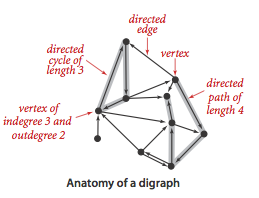
\includegraphics[width=1.0\linewidth,height=0.7\textheight]{../images/digraph-anatomy.png}
            \end{center}
         \end{column}
         \begin{column}{0.5\textwidth}
             \begin{center}
                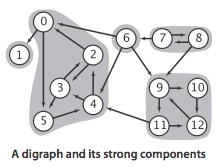
\includegraphics[width=1.0\linewidth,height=0.7\textheight]{../images/strong-components.png}
             \end{center}
        \end{column}
    \end{columns}
\end{frame}

\note[itemize]{
    \item The big takeaway here is the idea of ``edges'' and ``nodes''
    \item \href{https://algs4.cs.princeton.edu/42digraph/}{Source: Algorithms, 4th Edition, by Robert Sedgewick and Kevin Wayne}
    \item \href{https://www.youtube.com/watch?v=mXoiHgH4mEE}{Wrath of Math!}
}

\usebackgroundtemplate{
\includegraphics[width=\paperwidth]{../images/field.jpg}}
\section{What is Deep Learning, Exactly?}

\note[itemize]{
    \item You've probably heard this term lately, lets talk about what it means.
}

\usebackgroundtemplate{
\includegraphics[width=\paperwidth]{../images/tree.jpg}}
\begin{frame}{}
    \setlength{\TPHorizModule}{\textwidth}
    \setlength{\TPVertModule}{\textwidth}
    % Slide title in upper left
    \begin{textblock}{0.74} (0.05,0.05)
        \bfseries\large\textcolor{white}{The Rise of Deep Learning}
    \end{textblock}
    \bigskip
    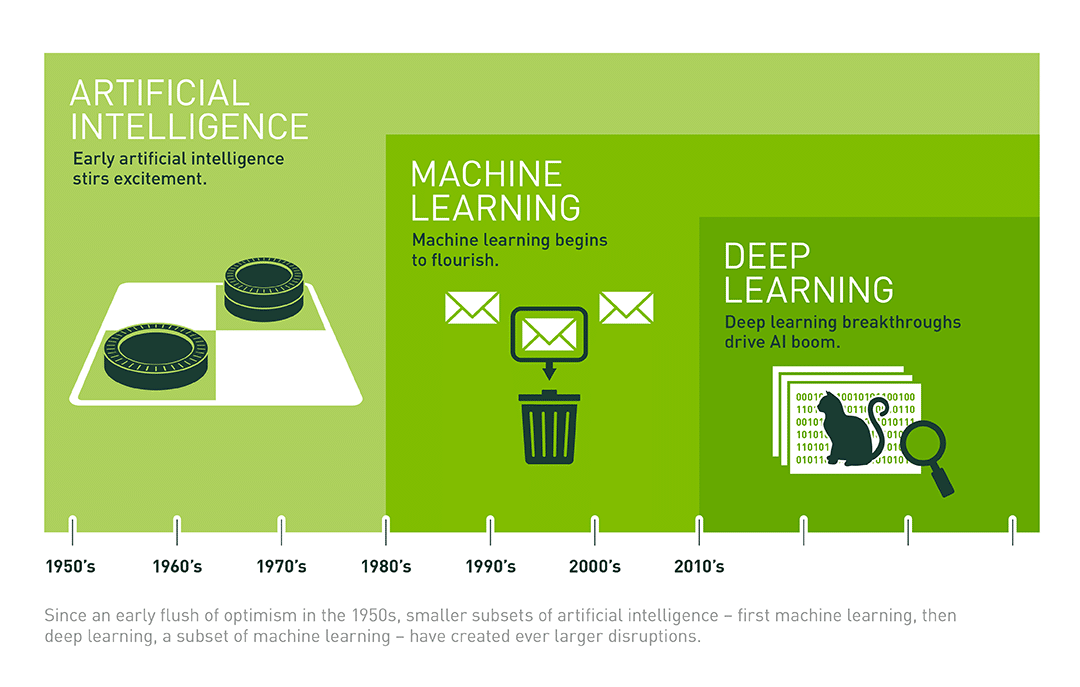
\includegraphics[width=1.0\linewidth,height=0.7\textheight]{../images/dl_timeline.png}

\end{frame}

\note[itemize]{
    \item GPUs have made it possible to expand accessibility to DL
    \item the CUDA toolkit from Nvidia has made things easier for researchers.
}

\usebackgroundtemplate{
\includegraphics[width=\paperwidth]{../images/tree.jpg}}
\begin{frame}{}
    \setlength{\TPHorizModule}{\textwidth}
    \setlength{\TPVertModule}{\textwidth}
    % Slide title in upper left
    \begin{textblock}{0.74} (0.05,0.05)
        \bfseries\large\textcolor{white}{Quick Intro to a Giant Topic}
    \end{textblock}
    \bigskip
    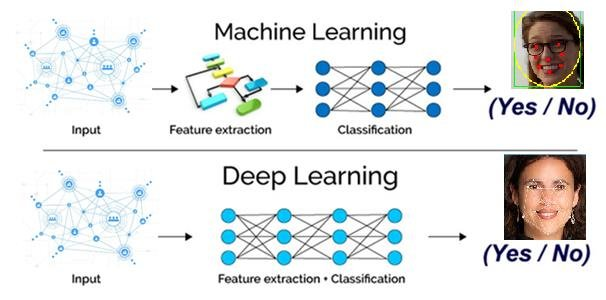
\includegraphics[width=1.0\linewidth,height=0.7\textheight]{../images/Diff-ML-DL.jpg}

\end{frame}

\note[itemize]{
    \item \href{https://www.researchgate.net/publication/338585724_Improved_Approach_for_Identification_of_Real_and_Fake_Smile_using_Chaos_Theory_and_Principal_Component_Analysis}{image source/credit}
    \item ML feature extraction can be a huge undertaking, up to 80\% of a project.
    \item DL attempts to automatically learn features that are most useful for a task from raw data.
    \item The nodes in a digraph are ``neurons'' or ``units'' in the DL/graph theory context.
    \item The neurons perform two steps. They calculate a ``weighted sum'' and pass the result through an ``activation function'' such as a rectifier activation function.
    \item These neurons or units that go through the rectifier function are called ``RelUs'' for short. Lot's of descriptive info in this one term!
    \item Depth of the GNN is measured by the number of connected layers.
    \item DL needs very large data sets for accurate feature determination. Data sets with lots of features are known as ``high density''.
    \item We humans interpret the features and output based on what we are trying to model.
}

\usebackgroundtemplate{
\includegraphics[width=\paperwidth]{../images/tree.jpg}}
\begin{frame}{}
    \setlength{\TPHorizModule}{\textwidth}
    \setlength{\TPVertModule}{\textwidth}
    % Slide title in upper left
    \begin{textblock}{0.74} (0.05,0.05)
        \bfseries\large\textcolor{white}{Amazing Training and Tools Available}
    \end{textblock}

    \begin{itemize}
        \item There is a ton of information suddenly. Books, papers, code, etc.
        \item Folks are very helpful, positioning themselves as experts.
        \item \href{https://youtu.be/8owQBFAHw7E}{super helpful videos like this one}
        \item The \href{https://developers.google.com/machine-learning/crash-course}{Google Machine Learning Crash Course} is free with tons of information.
    \end{itemize}

\end{frame}

\note[itemize]{
    \item Google Deep Learning Container Images
    \item Continuous Machine Learning (CML) Project
    \item Kaggle and shared Jupyter Notebooks
}

\usebackgroundtemplate{
\includegraphics[width=\paperwidth]{../images/field.jpg}}
\section{The Journey}
\note[itemize]{
    \item Now I would like to talk a bit about the shape of the project.
}

\usebackgroundtemplate{
\includegraphics[width=\paperwidth]{../images/tree.jpg}}
\begin{frame}{}
    \setlength{\TPHorizModule}{\textwidth}
    \setlength{\TPVertModule}{\textwidth}
    % Slide title in upper left
    \begin{textblock}{0.74} (0.05,0.05)
        \bfseries\large\textcolor{white}{What Have I Gotten Myself Into?}
    \end{textblock}
    \begin{columns}
    \begin{column}{0.5\textwidth}
        \begin{itemize}
            \item It didn't take long before I realized the magnitude of the ocean I was wading into.
            \item Started reading everything I could find even though I didn't understand most of it.
            \item I came up with the basic framework you see in the image here.
        \end{itemize}
    \end{column}
    \begin{column}{0.45\textwidth}
        \begin{center}
            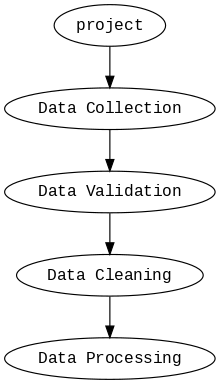
\includegraphics[width=1.0\linewidth, height=0.7\textheight]{../images/project.png}
        \end{center}
    \end{column}
\end{columns}
\end{frame}
\note[itemize]{
    \item Repetition can be a slow and painful way to learn.
    \item Wasn't even sure what questions to ask. Slow going at first.
}


\usebackgroundtemplate{
\includegraphics[width=\paperwidth]{../images/tree.jpg}}
\begin{frame}{}
    \setlength{\TPHorizModule}{\textwidth}
    \setlength{\TPVertModule}{\textwidth}
    % Slide title in upper left
    \begin{textblock}{0.74} (0.05,0.05)
        \bfseries\large\textcolor{white}{Yak Shaving, Side Quests, Endless Rabbit Holes}
    \end{textblock}
    % main body
    \begin{itemize}
        \item Makefiles and GNU Autotools
        \item NVIDA Jetson Nano as cluster nodes
        \item SLURM cluster scheduler
        \item OpenMPI for parallel builds
        \item Docker and Containers
        \item k8s and Rancher k3s
        \item Data Version Control \href{https://dvc.org}{dvc.org}
        \item Storing/accessing data in GCP buckets
        \item Continuous Machine Learning \href{https://cml.dev/}{cml.dev}
        \item Internal Pypi and Debian/Raspbian mirror (used too much bandwidth on home connection)
    \end{itemize}
\end{frame}

\note[itemize]{
    \item Wasn't sure exactly where to drop this slide in the order.
    \item Trying to show that there have been a TON of side quests.
    \item Some of these were useful, some led to spin off projects. A lot of this is bookmarked for later when I get some ``spare time'' haha.
}

\defverbatim[colored]\lstI{
    \begin{lstlisting}[language=Python,basicstyle=\ttfamily,keywordstyle=\color{red}]

        # Generate a PNG from Terraform
        terraform graph | dot -Tpng > graph.png

        # Generate vector graphic from Terraform
        terraform graph | dot -Tsvg -o graph.svg
    \end{lstlisting}
}

\usebackgroundtemplate{
\includegraphics[width=\paperwidth]{../images/tree.jpg}}
\begin{frame}{}
    \setlength{\TPHorizModule}{\textwidth}
    \setlength{\TPVertModule}{\textwidth}
    % Slide title in upper left
    \begin{textblock}{0.74} (0.05,0.05)
        \bfseries\large\textcolor{white}{Dot Data Collection}
    \end{textblock}
    \begin{itemize}
        \item A big barrier to entry was removed by the ability to output a Directed Graph from Terraform.
        \item \href{https://youtu.be/2FytVBJHUKk}{Click for video}
    \end{itemize}
    \lstI

\end{frame}

\note[itemize]{
    \item Was pretty happy I could generate a PNG file. Super easy!
    \item Then I opened up the file and took a look at the nodes in the graph....
}

\usebackgroundtemplate{
\includegraphics[width=\paperwidth]{../images/tree.jpg}}
\begin{frame}{}
    \setlength{\TPHorizModule}{\textwidth}
    \setlength{\TPVertModule}{\textwidth}
    % Slide title in upper left
    \begin{textblock}{0.74} (0.05,0.05)
        \bfseries\large\textcolor{white}{Python Data Collection}
    \end{textblock}
    \begin{columns}
    \begin{column}{0.5\textwidth}
        \begin{itemize}

        \item This became the basis for data collection via Python.
        \item Found a cool module on Pypi called \href{https://pypi.org/project/python-terraform/}{python-terraform} that allowed me to run Terraform CLI commands from inside Python.
        \item \href{https://youtu.be/aTE8uZVO248}{Click for video} %  % 2.5x python collection
        \end{itemize}
    \end{column}
    \begin{column}{0.5\textwidth}
    \begin{center}
    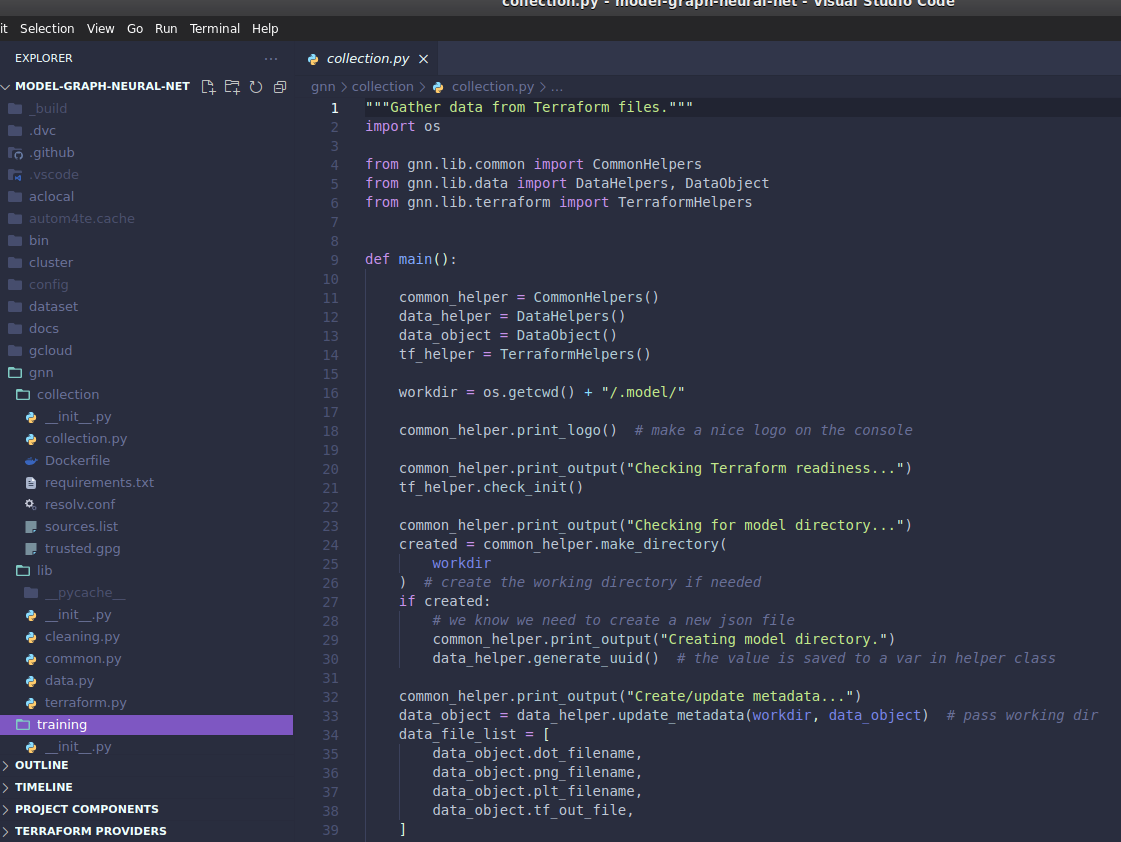
\includegraphics[width=1.0\linewidth, height=0.7\textheight]{../images/collection_code.png}
    \end{center}
    \end{column}
    \end{columns}
\end{frame}
\note[itemize]{
    \item Kind of a no brainer.
    \item The video is sped up 3x or so, but you can get the flavor of how the project looks from this.
}

\usebackgroundtemplate{
\includegraphics[width=\paperwidth]{../images/tree.jpg}}
\begin{frame}{}
    \setlength{\TPHorizModule}{\textwidth}
    \setlength{\TPVertModule}{\textwidth}
    % Slide title in upper left
    \begin{textblock}{0.74}(0.05,0.05)
        \bfseries\large\textcolor{white}{Data Processing Side Quest}
    \end{textblock}

    \begin{columns}
    \begin{column}{0.5\textwidth}
 \begin{itemize}
        \item This is what happens when you spend a week with P0lr.
     \end{itemize}
    \end{column}
    \begin{column}{0.5\textwidth}
        \begin{center}
    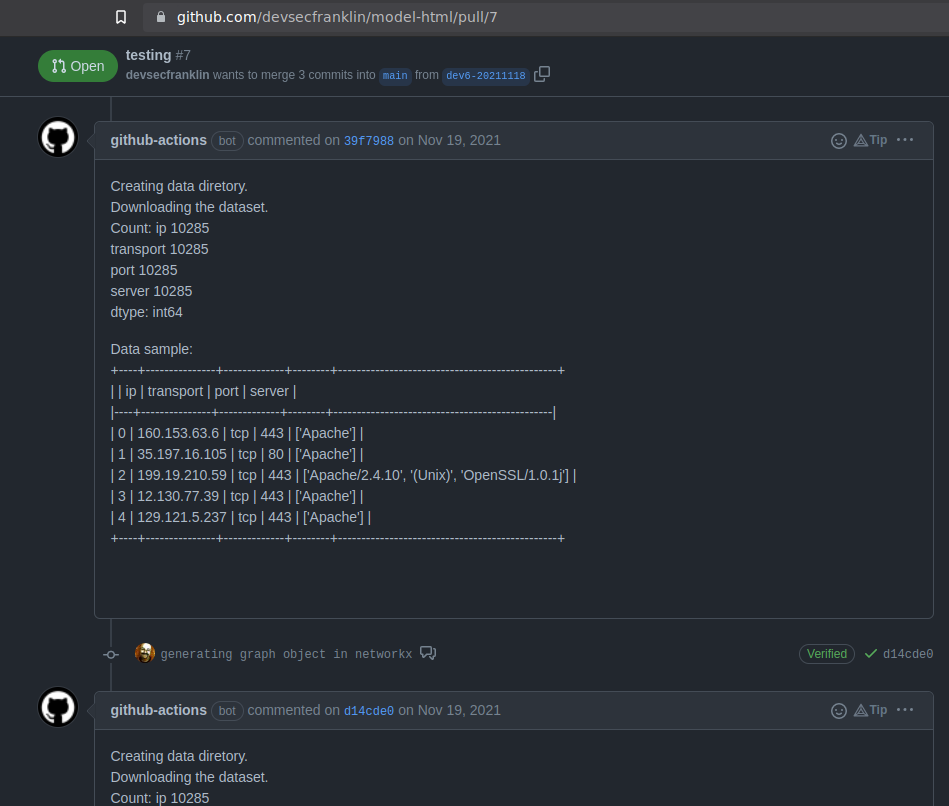
\includegraphics[width=1.0\linewidth,height=0.7\textheight]{../images/kaggle-cml.png}
\end{center}
    \end{column}
\end{columns}

\end{frame}
\note[itemize]{
    \item Spent a week with P0lr where we had a moderate case of machine learning fever.
    \item We had a direction but no destination.
    \item Watched Alpha Go movie, talked about a bunch of stuff, read some books and papers.
    \item wound up writing some code.
    \item there was a ``HTML model'' in there somewhere too
}

\usebackgroundtemplate{
\includegraphics[width=\paperwidth]{../images/tree.jpg}}
\begin{frame}{}
    \setlength{\TPHorizModule}{\textwidth}
    \setlength{\TPVertModule}{\textwidth}
    % Slide title in upper left
    \begin{textblock}{0.74}(0.05,0.05)
        \bfseries\large\textcolor{white}{Data Storage - Kaggle}
    \end{textblock}
    \begin{itemize}
    \item What the heck is it?
    \end{itemize}
\end{frame}
\note[itemize]{
    \item What the heck is it?
}

\usebackgroundtemplate{
\includegraphics[width=\paperwidth]{../images/tree.jpg}}
\begin{frame}{}
    \setlength{\TPHorizModule}{\textwidth}
    \setlength{\TPVertModule}{\textwidth}
    % Slide title in upper left
    \begin{textblock}{0.74}(0.05,0.05)
        \bfseries\large\textcolor{white}{Data Storage - Google Cloud}
    \end{textblock}

Data storage with GCP because it's (relatively) easy.
\end{frame}



\usebackgroundtemplate{
\includegraphics[width=\paperwidth]{../images/tree.jpg}}
\begin{frame}{}
    \setlength{\TPHorizModule}{\textwidth}
    \setlength{\TPVertModule}{\textwidth}
    % Slide title in upper left
    \begin{textblock}{0.74}(0.05,0.05)
        \bfseries\large\textcolor{white}{Data Storage - DVC}
    \end{textblock}
    \begin{itemize}
    \item Data storage and tagging using DVC
    \item \href{https://dvc.org/}{there is a video on this page that explains}
    \end{itemize}
\end{frame}


\usebackgroundtemplate{
\includegraphics[width=\paperwidth]{../images/tree.jpg}}
\begin{frame}{}
    \setlength{\TPHorizModule}{\textwidth}
    \setlength{\TPVertModule}{\textwidth}
    % Slide title in upper left
    \begin{textblock}{0.74}(0.05,0.05)
        \bfseries\large\textcolor{white}{Data Pipeline}
    \end{textblock}

    \begin{columns}
    \begin{column}{0.5\textwidth}
        \begin{itemize}
            \item The Data Pipeline is a set of processes that move and transform data from various sources to a destination where new value can be derived.
            \item The DP is the foundation of analytics, reporting, and machine learning capabilities.
        \end{itemize}
    \end{column}
    \begin{column}{0.45\textwidth}
        \begin{center}
            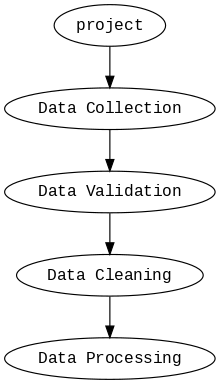
\includegraphics[width=1.0\linewidth, height=0.7\textheight]{../images/project.png}
        \end{center}
    \end{column}
\end{columns}
\end{frame}

\note[itemize]{
    \item Source: Data Pipelines pocket reference p1-2
}

\usebackgroundtemplate{
\includegraphics[width=\paperwidth]{../images/field.jpg}}
\section{Visualizations}

\usebackgroundtemplate{
\includegraphics[width=\paperwidth]{../images/tree.jpg}}
\begin{frame}{}
    \setlength{\TPHorizModule}{\textwidth}
    \setlength{\TPVertModule}{\textwidth}
    % Slide title in upper left
    \begin{textblock}{0.74}(0.05,0.05)
        \bfseries\large\textcolor{white}{Graphviz/Dot output}
    \end{textblock}

    \begin{textblock}{0.75}(0.025,0.08)
        \bigskip
        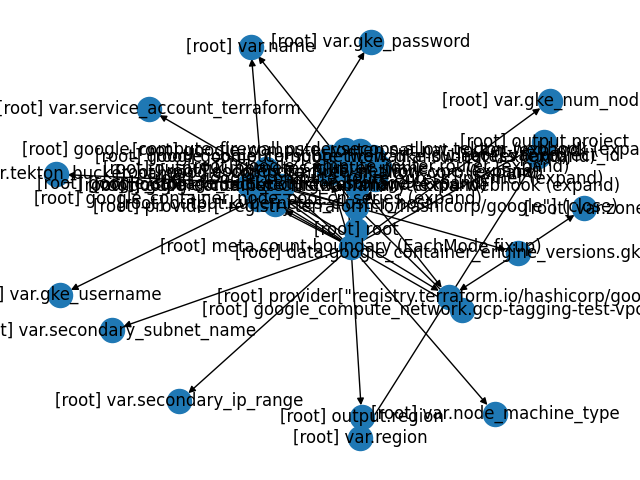
\includegraphics[width=1.0\linewidth,height=0.7\textheight]{../images/graph-dl-test}
    \end{textblock}
\end{frame}
\note[itemize]{
    \item This is the first thing I saw when I started converting the data.
    \item Was excited here since I was able to change the color of the nodes.
    \item Obviously this is not yet a usable result
    \item \href{https://youtu.be/mmHBexAHNa4}{some video of data collection}
}

%\usebackgroundtemplate{
\includegraphics[width=\paperwidth]{../images/tree.jpg}}
%\begin{frame}{}
%    \setlength{\TPHorizModule}{\textwidth}
%    \setlength{\TPVertModule}{\textwidth}
%    % Slide title in upper left
%    \begin{textblock}{0.74}(0.05,0.05)
%        \bfseries\large\textcolor{white}{Gephi}
%    \end{textblock}
%
%\end{frame}


%\usebackgroundtemplate{
\includegraphics[width=\paperwidth]{../images/field.jpg}}
%\section{But, I Heard There was Math?}
%
%\usebackgroundtemplate{
\includegraphics[width=\paperwidth]{../images/tree.jpg}}
%\begin{frame}{}
%    \setlength{\TPHorizModule}{\textwidth}
%    \setlength{\TPVertModule}{\textwidth}
%    % Slide title in upper left
%    \begin{textblock}{0.74}(0.05,0.05)
%        \bfseries\large\textcolor{white}{The training.py Part}
%    \end{textblock}
%
%    \begin{itemize}
%        \item As the number of nodes and edges in the graph increase, it becomes more difficult to visualize the graph diagrammatically.
%        \item Graph data in a tabular matrix-style layout is possible.
%    \end{itemize}
%\end{frame}
%
%\note[itemize]{
%    \item Created a separate piece of Python where I intend to do some ``training''
%    \item Does some Linear Algebra operations on some matrices so far.
%}

\usebackgroundtemplate{
\includegraphics[width=\paperwidth]{../images/tree.jpg}}
\begin{frame}
    \setlength{\TPHorizModule}{\textwidth}
    \setlength{\TPVertModule}{\textwidth}
    % Slide title in upper left
    \begin{textblock}{0.74}(0.05,0.05)
        \bfseries\large\textcolor{white}{The Adjacency Matrix}
    \end{textblock}

    \begin{itemize}
    \item Let G be a graph with n vertices that are assumed to be ordered from \[ v_1\] to \[ v_n \].
    \end{itemize}
    The n x n matrix A, in which

    \[ a_{ij} = 1 \] if there exists a path from \[ v_i \] to \[v_j \]
    \[ a_{ij} = 0 \] otherwise

    is called an adjacency matrix.
\end{frame}

%\note[itemize]{
%\item There is an Incidence Matrix, and a dense Incidence matrix.
%\item Consider the \href{http://ceadserv1.nku.edu/longa//classes/mat385_resources/docs/matrix.html}{information at this link}.
%
%    \item The first type of Matrix layout is the Adjacency Matrix.
%    \item There is an Adjacency Matrix, and also a ``dense'' version of the Adjacency Matrix.
%}
%
%\usebackgroundtemplate{
\includegraphics[width=\paperwidth]{../images/tree.jpg}}
%\begin{frame}{}
%    \setlength{\TPHorizModule}{\textwidth}
%    \setlength{\TPVertModule}{\textwidth}
%    % Slide title in upper left
%    \begin{textblock}{0.74}(0.05,0.05)
%        \bfseries\large\textcolor{white}{The Incidence Matrix}
%    \end{textblock}
%    \begin{itemize}
%        \item Let G be a graph with n vertices that are assumed to be ordered from v_1 to v_n.
%    \end{itemize}
%\end{frame}
%\note[itemize]{
%    \item
%}

%\usebackgroundtemplate{
\includegraphics[width=\paperwidth]{../images/tree.jpg}}
%\begin{frame}{}
%    \setlength{\TPHorizModule}{\textwidth}
%    \setlength{\TPVertModule}{\textwidth}
%    % Slide title in upper left
%    \begin{textblock}{0.74}(0.05,0.05)
%        \bfseries\large\textcolor{white}{The Laplacian Matrix}
%    \end{textblock}
%
%\end{frame}

\usebackgroundtemplate{
\includegraphics[width=\paperwidth]{../images/field.jpg}}
\section{So Now What?}

\usebackgroundtemplate{
\includegraphics[width=\paperwidth]{../images/tree.jpg}}
\begin{frame}{}
    \setlength{\TPHorizModule}{\textwidth}
    \setlength{\TPVertModule}{\textwidth}
    % Slide title in upper left
    \begin{textblock}{0.74}(0.05,0.05)
        \bfseries\large\textcolor{white}{Useful Intermediate Results}
    \end{textblock}
    % main body bullet points
    \begin{itemize}
        \item Standardizing my data collection on JSON.
        \item Made some super cool functions for parsing nested JSON.
        \item Turned some of this time into money with \href{https://youtu.be/U62scNwsvc0}{cloud tools}
        \item Importing JSON to Pandas dataframes.
    \end{itemize}
\end{frame}
\note[itemize]{
    \item Tabular data in Pandas can be output in all kinds of formats.
    \item Pandas data frames can be the input for other Machine Learning tools and frameworks.
}

\usebackgroundtemplate{
\includegraphics[width=\paperwidth]{../images/tree.jpg}}
\begin{frame}{}
    \setlength{\TPHorizModule}{\textwidth}
    \setlength{\TPVertModule}{\textwidth}
    % Slide title in upper left
    \begin{textblock}{0.74}(0.05,0.05)
        \bfseries\large\textcolor{white}{Next Steps for this Project}
    \end{textblock}
    % main body bullet points
    \begin{itemize}
        \item The data collection problem (Don't have access to enough data!)
        \item Maybe have a ``collection container'' with a python/Flask RESTful API for folks to push data to? Or even better, scrape GH for public repos with Terraform? (Lots of data, but not all security infra)
        \item Maybe back to Kaggle to find some big data to operate on?
        \item See if I can get the training to use my personal GPU/TPU.
    \end{itemize}
\end{frame}
\note[itemize]{
    \item Most of this work is relegated to my ``free'' time.
    \item Have to spend my days helping people with the cloud.
}

%\usebackgroundtemplate{
\includegraphics[width=\paperwidth]{../images/tree.jpg}}
%\begin{frame}{}
%    \setlength{\TPHorizModule}{\textwidth}
%    \setlength{\TPVertModule}{\textwidth}
%    % Slide title in upper left
%    \begin{textblock}{0.74}(0.05,0.05)
%        \bfseries\large\textcolor{white}{If Time, Staff, and Money were no Object}
%    \end{textblock}
%    % main body bullet points
%    \begin{itemize}
%        \item Dreams and stretch goals.
%    \end{itemize}
%\end{frame}
%\note[itemize]{
%    \item this is the ``dreams and stretch goals'' slide.
%    \item Most of this work is relegated to my ``free'' time.
%    \item Have to spend my days helping people with the cloud.
%}

%\usebackgroundtemplate{
\includegraphics[width=\paperwidth]{../images/tree.jpg}}
%\begin{frame}{}
%    \setlength{\TPHorizModule}{\textwidth}
%    \setlength{\TPVertModule}{\textwidth}
%    % Slide title in upper left
%    \begin{textblock}{0.74} (0.05,0.05)
%        \bfseries\large\textcolor{white}{Data Collection Container}
%    \end{textblock}
%
%\end{frame}
%
%\note[itemize]{
%    \item A containerized (web?) app for folks to submit Terraform plans.
%}

\usebackgroundtemplate{
\includegraphics[width=\paperwidth]{../images/field.jpg}}
\section{Sources and Citations}

\usebackgroundtemplate{
\includegraphics[width=\paperwidth]{../images/tree.jpg}}
\begin{frame}{}
    \setlength{\TPHorizModule}{\textwidth}
    \setlength{\TPVertModule}{\textwidth}
    % Slide title in upper left
    \begin{textblock}{0.74}(0.05,0.05)
        \bfseries\large\textcolor{white}{Sources and Citations}
    \end{textblock}
    % main body bullet points
    \begin{itemize}
        \item Generate a bibtex
    \end{itemize}
\end{frame}
\note[itemize]{
    \item Need to add a reading list on here
    \item Make a list of all the books and papers
}

\end{document}
